\chapter{Implementación}
\label{cap:implementacion}

En éste capítulo introduciremos los detalles mas relevantes del desarrollo realizado para este trabajo. Comenzaremos mostrando la integración de nuestro sistema de NLG con \textit{Fastest}, viendo el modo de uso y los nuevos comandos introducidos para la generación de descripciones en lenguaje natural. Luego presentaremos los aspectos mas destacados de nuestra implementación para cada una de las etapas del \emph{pipeline}.

\section{Integración con \emph{Fastest}}

La implementación realizada para este trabajo se encuentra incluida en la última versión de \emph{Fastest}, que puede ser descargada de TODO. El código de esta, así como también el desarrollo realizado para este trabajo se halla disponible públicamente en https://github.com/rosacris/fastest, encontrando la mayor parte del código referente a este trabajo dentro del paquete \textit{main.java.nlg}.

\subsection*{Requisitos}

Deberemos cumplir con los siguientes requerimientos a fin de garantizar el correcto funcionamiento de nuestro sistema de NLG:
\begin{itemize}
 \item  \emph{Fastest 1.7 o superior \footnote{http://todo/}}: La distribución de este incluye un pequeño manual de uso.
 \item  \emph{Java SE Runtime Environment 1.6 o superior}: requerido para el correcto funcionamiento de \emph{Fastest}.
 \item  \emph{SWI-Prolog \footnote{http://http://www.swi-prolog.org/}}: también requerido para el correcto funcionamiento de Fastest.
 \item  \emph{FreeLing 3.1 \footnote{http://nlp.lsi.upc.edu/freeling/}\footnote{Pequeño tutorial para la instalación de \emph{FreeLing} en \emph{Ubuntu 15.04}: https://gist.github.com/juliandt/8a364d75d8b271c698aa}}: suite de análisis de lenguajes, necesaria para el módulo de NLG de \emph{Fastest}
\end{itemize}

\section{Arquitectura}

\subsection{\textit{Document Planner}}

El módulo \emph{DocumentPlanner} será el encargado de llevar a cabo las tareas de determinación de contenido y estructuración del documento detalladas en el capítulo \ref{cap:document_planning}. En la figura \ref{fig:dp_classes} podemos observar los componentes mas importantes involucrados en esta etapa. 

\begin{figure}[H]
  	\centering
	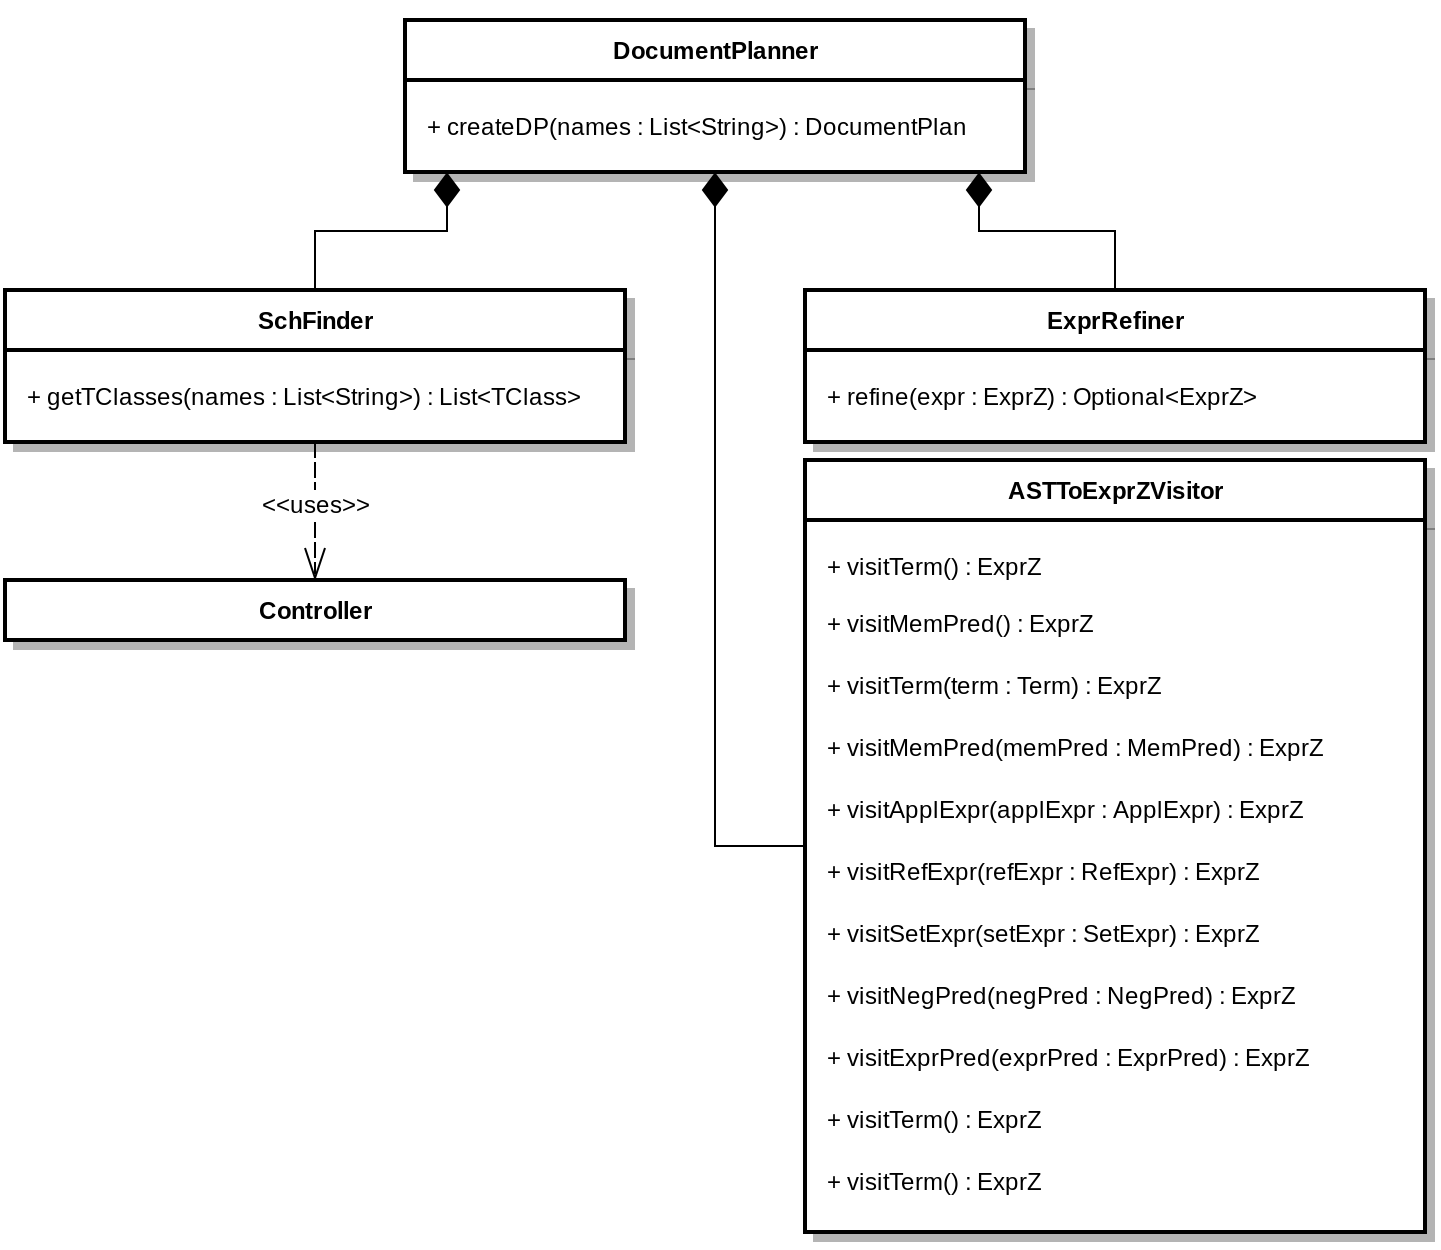
\includegraphics[scale=0.25]{img/dp_classes.png}
	\caption{Diagrama clases \textid{DocumentPlanner}
  	\label{fig:dp_classes}
\end{figure}

La tarea de selección es delegada en el módulo \emph{SchFinder} utilizado por el \emph{DocumentPlanner}. Este será el encargado de recuperar el conjunto de clases de prueba indicadas. El mismo posee una referencia al \emph{Controller} \footnote{Es el módulo encargado de mantener las referencias a elementos de la especificación, arboles de prueba, etc.} de Fastest que le permitirá identificar y recuperar las clases de prueba necesarias. 

Por otro lado, las tareas de eliminación de tautologías y reducción de expresiones se encuentran encapsuladas detrás de la fachada \emph{ExprZRefiner} encargada de delegar los distintos procesamientos a realizar sobre las expresiones. Podemos notar que utilizamos la clase \emph{Optimal} de Java 8 para modelar el hecho de que el método \textbf{refine()} podría no devolver un valor, por ejemplo en el caso que la expresión procesada sea una tautología y no deba ser incluida en el \textit{document plan}.

Fastest utiliza el \textit{framework} CZT \footnote{http://czt.sourceforge.net/} que integra un conjunto de herramientas para trabajar con el lenguaje de especificación Z. La forma en la que CZT modela las expresiones de Z nos resultó demasiado compleja para este trabajo, por lo que decidimos transformar las expresiones contempladas dentro del alcance de este trabajo a un modelo más simple (los que nos simplificará posteriormente la implementación del algoritmo de lexicalización, por ejemplo). En la figura \ref{fig:exprz_classes} podemos observar la jerarquía de clases de las expresiones utilizadas en este trabajo para modelar las expresiones Z. 

\begin{figure}[H]
  	\centering
	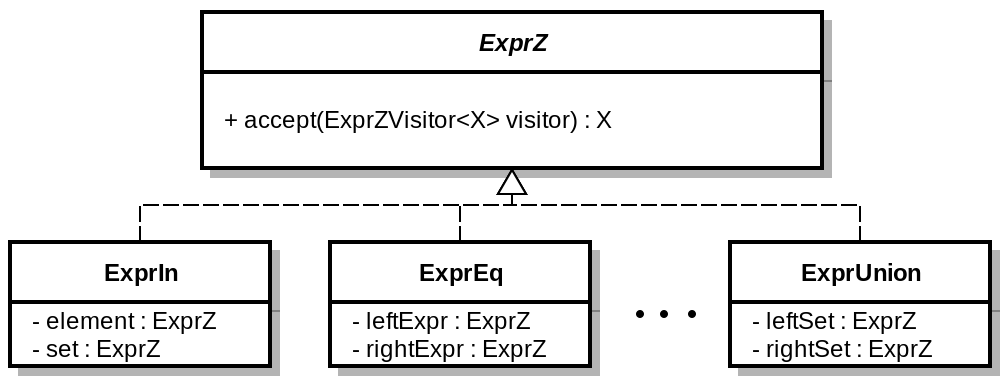
\includegraphics[scale=0.3]{img/exprz_classes.png}
	\caption{Diagrama jerarquía de clases ExprZ}
  	\label{fig:exprz_classes}
\end{figure}

Es el módulo \emph{ASTToExprZVisitor} el responsable de esta transformación entre el modelo de CZT y el utilizado por este trabajo.

\subsection{\textit{Microplanner}}

\subsection{\textit{Surface Realizer}}